\chapter{Future Work}
\label{chap:future}

\newcommand{\llm}{LLM\xspace}
\newcommand{\llmfull}{Large Language Model\xspace}
\newcommand{\kv}{KV\xspace}
\newcommand{\kvfull}{key-value\xspace}
\newcommand{\kvcache}{\kv cache\xspace}
\newcommand{\kvcachefull}{\kvfull cache\xspace}
\newcommand{\gptfast}{gpt-fast\xspace}
\newcommand{\cxl}{CXL\xspace}
\newcommand{\cxlfull}{Compute Express Link\xspace}
\newcommand{\api}{API\xspace}
\newcommand{\gpu}{GPU\xspace}
\newcommand{\ssd}{SSD\xspace}
\newcommand{\slo}{SLO\xspace}
\newcommand{\slofull}{service-level objective\xspace}
\newcommand{\roifull}{Return on Investment\xspace}
\newcommand{\roi}{ROI\xspace}
\newcommand{\apisave}{\texttt{save}\xspace}
\newcommand{\apiload}{\texttt{load}\xspace}
\newcommand{\ttft}{TTFT\xspace}
\newcommand{\ttftfull}{time to first token\xspace}
\newcommand{\llama}{LLaMA\xspace}
\newcommand{\asic}{ASIC\xspace}

\newcommand{\tool}{\textit{KVExpress}\xspace}

\newcommand{\sam}[1]{{\color{blue}#1}\xspace}
\newcommand{\ltp}[1]{{\color{magenta}#1}\xspace}
\newcommand{\Space}[1]{\xspace}
\newcommand{\fix}[1]{{\color{red}#1}\xspace}

\newcommand{\para}[1]{\vspace{3pt}\noindent \textbf{#1.}~~}


\section{Introduction}
Autoregressive large language models generate output tokens sequentially, where the generation of each token involves computing attention with \kvfull (\kv) data of all the preceding tokens~\cite{gpt1, gpt2, gpt3}. 
This sequential dependency has make \llm inference both compute- and memory-intensive~\cite{gpt4}.
\llm inference typically has two stages: (1) the prefill stage, where all input tokens are processed (in parallel) to generate the initial output token, and (2) the decode stage, where the rest of the output tokens are generated one by one until the model generates an end-of-sequence token. 


For applications such as chatbot and coding assistant, \llm serving systems aim to minimize the time to finish the prefill stage, or \ttftfull (\ttft).
In production, \slofull (\slo) for \ttft is typically 400ms ~\cite{distserve}.
To meet such \slo, \llm serving systems often cache the previously-computed \kv data of preceding tokens (i.e., prefix) in GPU memory\Space{ incurred from the attention mechanism}, to avoid re-computing them for future requests that have the same prefix~\cite{pagedattenion, distserve, memserve}. 
Storing \kvcache reduces the overall computational load and significantly improves throughput by trading memory for computation. 


In production chatbot applications that support large context window, the demand for \kvcache storage grows rapidly by the amount of inference requests from users, which cannot be accommodated sheerly by the limited, expensive GPU memory.
Researchers thus developed techniques to offload \kvcache to CPU memory, leveraging the larger CPU memory capacity to reduce GPU memory pressure~\cite{pagedattenion, memserve, cacheblend}. 
However, as larger \llm{}s and support for long-context inference requests continue to emerge, the approach of offloading to CPU memory becomes more limited.
For example, in \llama-2-7B, \kvcache of token in FP32 precision is 1024KB; \kv cache of a single request with 4096 tokens (maximum context length) is 4GB~\cite{llama2}.
\Space{As models scale and support longer contexts—some even up to 2 million tokens—a single request could theoretically consume as much as 2TB of memory just for KV cache.}
The memory demand from serving many concurrent long-context requests can easily overwhelm even high-end memory servers~\cite{pagedattenion, kvcost}. 

Practitioners increasingly turn to more scalable memory architectures, such as \cxlfull (\cxl) memory~\cite{cxl1, cxl2, pond}, to address the growing memory demands of large-scale systems. 
\cxl{}\Space{ is an emerging technology that} expands memory capacity by connecting additional DRAM to servers via PCIe, while maintaining low-latency access. It offers a promising solution to the \kvcache storage demand in \llm serving.

\fix{
In this paper, we propose to leverage \cxl memory for offloading \kvcache, with the goal to improve serving throughput while retaining \slo on \ttft, and reduce memory pressure for the upper-level \llm serving system. This paper makes the following contributions:
\Space{to alleviate memory pressure, improve scalability, and enhance overall performance of the target \llm serving system.
to improve efficiency to handle larger context lengths, process more concurrent requests while adhering to \slo, and improve resource allocation, improving both performance and scalability.
In this paper, we propose leveraging CXL memory to store KV caches, with a particular focus on the \ltp{the definition of prefix kv cache is not precise: prefix KV cache, which retains the keys and values of previously generated tokens during LLM inference}. By utilizing CXL memory, we aim to alleviate memory pressure, improve scalability, and enhance overall system performance. Our key contributions are as follows:
}
\begin{itemize} 
\item\Space{ \textbf{Preliminary Evaluation:}} We present the first measurement of \cxl-GPU interconnect and evaluate its feasibility for \kvcache offloading. \Space{, showcasing its potential to meet performance demands.} We show that \fix{XXX}. 
\item\Space{ \textbf{CXL-based KV Cache Management System:}} We describe our initial design of \cxl-based \kvcache offloading interface and present its performance evaluation for \llm serving, on our hardware platform that is the first to successfully integrate \asic-\cxl device and GPU.
\item\Space{ \textbf{Exploring Trade-offs and Future Directions:}} We examine the trade-offs in using \cxl for \kvcache offloading (\S\ref{?}) with \roifull (\roi) modeling, and identify promising areas for future research and development.
\end{itemize}
}

\section{\cxl-based \kv Cache Offloading}
\label{sec:implementation}

We now present the design and implementation of our \cxl-based \kvcache offloading interface for \llm serving. We also describe the hardware platform used to evaluate our design.

\para{Design and implementation} Our goal is to develop a \cxl storage interface, named \tool, which can be integrated into existing \llm serving systems for saving and loading \kvcache of inference requests.
\tool provides two external \api{}s to its upper-level serving system: \apisave and \apiload. 
The \apisave takes an unique identifier of a token chunk as input, and copies its \kvcache from \gpu to \cxl memory. 
The \apiload takes an unique identifier of a token chunk as input, and finds if its  \kvcache exists in \cxl memory, if so, copies the \kvcache from \cxl memory to \gpu. A token chunk can consist of one or more tokens.
The unique identifier of a token chunk $t_i$ for a sequence is the hash of the content of $t_i$ and the hash of its prefix $\langle t_0,...,t_{i-1}\rangle$. If the prefix of a sequence of a current request has been computed and saved into \cxl, \tool will load the \kvcache of the prefix from \cxl and use it when computating for this request\Space{, and use it when computing the rest of the input sequence}~\cite{pagedattenion}. 

To avoid calling \apisave and \apiload too frequently and incurring unnecessary overhead to the upper-level serving system, \apisave is called only when a request finished so the \kvcache of all the tokens for that request is saved at once; \apiload is called for a request prior to its prefill computation. 
\Space{
\tool also performs memory tiering. When \cxl memory is filled, the least recently accessed \kvcache{}s are evicted to persistent storage of the server, e.g., \ssd.
\tool tracks the metadata of all saved \kvcache{}s.
In \apiload, if a lookup in the \cxl memory is unsuccessful, \tool will perform lookup in the lower tier storage, if the lookup is then successful, \tool will transfer the data from lower tier storage to both \cxl and \gpu.
An evicted \kvcache{} will not be automatically transferred back to the \cxl memory even if there is enough space in the \cxl.
Lastly, to avoid overhead of data transfer due to frequent evictions, the eviction mechanism regularly evicts a fixed ratio of \kvcache{}s in \cxl--the ratio is calculated as a user-configured percentage of the total \cxl memory capacity.
}

We implement our design of \tool in \gptfast~\cite{gpt-fast}, a simple and low-latency text generation system with support on a number of widely-used inference optimizations and \llm. 
We further modify \gptfast to support our evaluation on batched inference.

\para{Hardware platform} 
Our single socket server is equipped with Intel Xeon Platinum processors~\cite{intelplatinum}, 1TB of 4800 MHz DDR5 memory, an NVIDIA H100 GPU with 96GB HBM, and a CXL memory expansion card with 256 GB of DDR5 memory at 4800 MHz. 
While prior works~\cite{cxlgpu1, cxlgpu2, cxlgpu3} have explored utilizing CXL for accelerators, to our knowledge, our work is the \textbf{first implementation to successfully integrate a real ASIC-CXL device and a GPU within a single inference server}.

\section{Performance Evaluation}
\label{sec:eval}

In Section~\ref{sec:eval:connect}, we measure the latency and bandwidth of \cxl-GPU interconnect for data transfer to assess the feasibility of storing \kvcache on \cxl devices.
In Section~\ref{sec:eval:ttft}, we compare the \ttft of \kv re-compute, prefix caching with \cxl, and prefix caching with GPU, to understand if \tool can achieve similar \ttft as existing approaches for prefill requests under varying context lengths.
In Section~\ref{sec:eval:throughput}, we study the maximum batch size achieved while retaining a given \slo on \ttft between \kv re-compute and prefix caching with \cxl.
\Space{Our evaluation is divided into three parts: (1) We present comprehensive latency and bandwidth results for data transfers between the GPU and the CXL device, assessing the feasibility of storing KV Cache on CXL devices. (2) We compare the Time to First Token (TTFT) across different approaches during the prefill stage. (3) We evaluate the maximum batch size achievable under a specified SLO when using either GPU compute or CXL storage.}


\begin{figure*}[ht!]
    \centering
    \subfigure[\cxl-GPU interconnect]{
    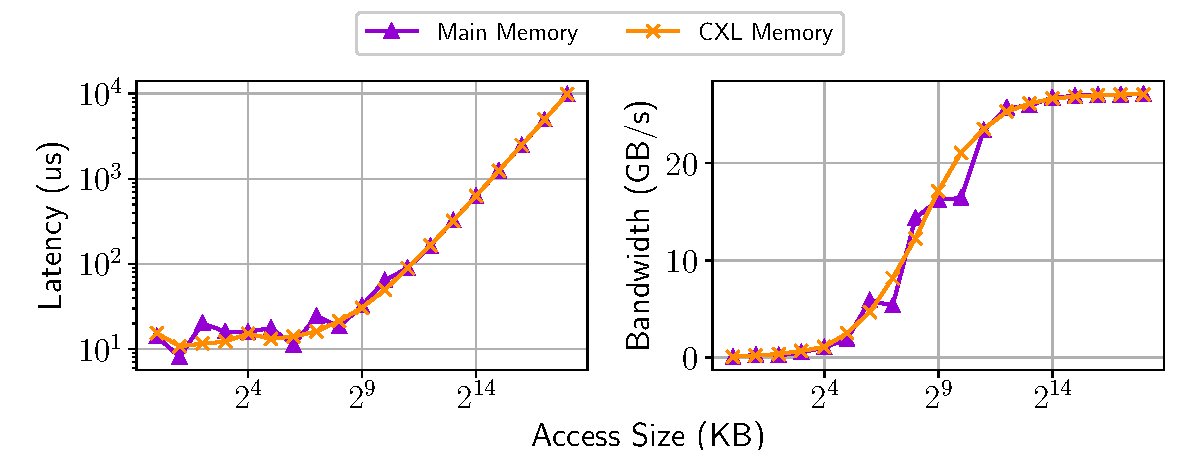
\includegraphics[width=0.47\textwidth]{fig/future/latency_bandwidth_vs_access_size.pdf}
        \label{fig:interconnect}
    }
    \subfigure[\ttft Comparison]{
        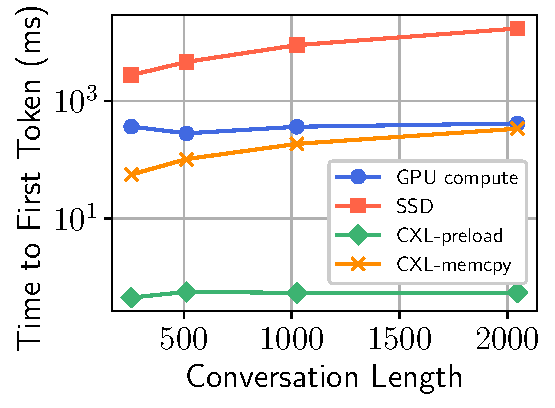
\includegraphics[width=0.23\textwidth]{fig/future/performance_comparison_logscale.pdf}
        %\vspace{1pt}
        \label{fig:performance}
    }
    \subfigure[Max BS under SLO]{
        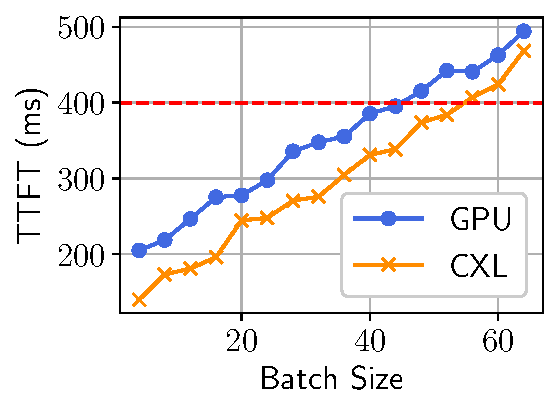
\includegraphics[width=0.23\textwidth]{fig/future/batch.pdf}
        \label{fig:batch}
    }
    \vspace{-1em}
    \caption{\textbf{\Space{Feasibility of caching KVcache in CXL memory pool.}Experiment results.} \fix{Please use the same y-axis title for (b) and (c)}} 
    \label{fig:evaluation}%\vspace{-1.5em}
\end{figure*}


\subsection{Measurements on CXL-GPU interconnect performance}
\label{sec:eval:connect}

\kvcache storage requires low-latency access (e.g., from host memory to GPU memory). 
Although prior studies~\cite{cxl1, cxl2} show that accessing \cxl memory from the host CPU is over $2\times$ slower than accessing local memory, none of their measurements involves any interaction with the GPU. 
In this paper, we evaluate the\Space{ basic} performance characteristics of the \cxl-GPU interconnect by measuring the latency and bandwidth of copying data from \cxl memory to the GPU. Transferring in the reverse direction yields similar results.
Since \cxl memory devices are exposed to the system as NUMA nodes without CPUs by default~\cite{cxl2}, we allocate a set of host buffers on the \cxl NUMA node and use \texttt{cudaMemcpyAsync} to copy data between the host buffers and GPU device buffers allocated via the CUDA API. 
We evaluated transferring data of size ranging from 1KB to 256MB.

Figure~\ref{fig:interconnect} shows our experiment results: the performance of the \cxl-GPU interconnect is \textit{unexpectedly} on par with traditional CPU-GPU memory transfers, exhibiting no significant slowdown. 
Latency remains low for smaller access sizes but increases exponentially once the size exceeds 64KB. 
Meanwhile, bandwidth increases almost linearly with data size and saturates around 4MB. 
This indicates that, while the CPU oversees the data transfer, the data path actually bypasses the host's local memory, flowing directly from CXL memory to GPU buffers via PCIe.\Space{\ltp{the data path bypasses an additional copy to the host's local memory, flowing directly from CXL memory to GPU buffers via PCIe.}\ltp{the data path actually bypasses the host's local memory, flowing directly from CXL memory to GPU buffers via PCIe.}}
Our results demonstrate that the CXL-GPU interconnect operates efficiently with minimal latency overhead, positioning it as a promising storage expansion in addition to CPU memory for \kvcache{} offloading\Space{ in large-scale systems}.

% \subsection{Feasibility of CXL-based Prefill Stage}
\subsection{Evaluation on \ttft under varying input context length}
\label{sec:eval:ttft}

Given that \cxl-GPU interconnect performs nearly the same as CPU-GPU interconnect, we further study if \cxl-based \kvcache offloading can achieve similar \ttft as existing approaches in completing the prefill stage computation for an inference request. 
We evaluate three approaches:
\begin{itemize} 
\item \textbf{\kv re-compute}: compute \kv data of all input tokens for the request with GPU. 
\item \textbf{Prefix caching with \cxl}: load \kvcache of the prefix tokens for the request from \cxl to GPU. 
% Load the entire conversation onto the GPU and compute the KV Cache from the scratch on the GPU. 
\item \textbf{Prefix caching with GPU}: store and use \kvcache in GPU for the prefix tokens for the request.\Space{This is the original CXL preload approach}
\item \fix{\textbf{Prefix caching with SSD}: load \kvcache of the prefix tokens for the request from SSD to GPU.} \sam{REMOVE IF THIS APPROACH DOES NOT EXIST IN PRIOR WORK} 
\end{itemize}
\Space{Given that the CXL-GPU interconnect exhibits similar performance characteristics to the CPU-GPU interconnect, the next question we address is whether it is feasible to meet SLO requirements by storing the KV Cache in CXL memory rather than recomputing it during the prefill stage.
We compared four methods: 
\begin{itemize} 
\item \textbf{GPU Compute}: Load the entire conversation onto the GPU and compute the KV Cache from the scratch on the GPU. 
\item \textbf{SSD}: Store the KV Cache on SSD; when serving a new request, load the KV Cache from the SSD to GPU memory and proceed to the decode stage. 
\item \textbf{CXL-Preload}: Store the KV Cache in CXL memory, preload it to the GPU memory before serving the corresponding inference request, and then directly proceed to decoding. 
\item \textbf{CXL-Memcpy}: Store the KV Cache in CXL memory, and load the KV Cache to GPU memory on-the-fly during the request. 
\end{itemize}}

% \ltp{It seems to me that CXL-Preload does not add much value here. Maybe we should remove it, or name it as ``Preload-Only''. Actually, it does not matter whether it is loaded from CXL or CPU memory. We should remove it if space is not sufficient. }\sam{ack}
% \ltp{It is a little bit controversal to add ''SSD'' here, as there is a way to utilize GPU-direct to access SSD as well. I am fine to keep it or remove it. }\sam{ack}
We measure the \ttft of the aforementioned approaches on conversation requests of input length ranging from 256 to 2048 tokens from the ShareGPT-Vicuna-Unfiltered dataset~\cite{dataset}.
\fix{We use the \llama-2-7B as the underlying model for all our experiment.}
% We selected multiple conversations of varying lengths (256–2048 tokens) from the ShareGPT\_Vicuna\_unfiltered dataset~\cite{dataset} and measured the TTFT for each conversation length. 
Figure~\ref{fig:performance} shows the \ttft (y-axis in log-scale) achieved by the evaluated approaches for requests of varying input context length (x-axis). 
% Figure~\ref{fig:performance} (Y-axis in log-scale) shows the results.

Compared to the other approaches, prefix caching with GPU (denoted as ``PC-GPU'' in Figure~\ref{fig:performance}) achieves the smallest \ttft (\fix{XXX}ms to \fix{XXX}ms) constantly across different input context lengths. Such performance is expected as there is no data transfer latency and computation of \kv data is only needed for tokens after the prefix. 
This approach is an optimal baseline that is however difficult to achieve in practice due to limited memory capacity of existing GPU models.
\fix{Prefix caching with SSD (denoted as ``PC-SSD'') yields the worse performance, with achieved \ttft ranging from \fix{XXX}ms to \fix{XXX}ms, because loading \kvcache takes over a second due to the slow access speed of \ssd.}\sam{REMOVE IF THIS APPROACH DOES NOT EXIST IN PRIOR WORK}

Comparing prefix caching with \cxl (denoted as ``PC-\cxl'') and \kv re-compute, prefix caching with \cxl performs at least as good as computing \kv data on GPU from scratch. Prefix caching with \cxl achieve \ttft ranging from \fix{XXX}ms to \fix{XXX}ms, with slight increase in latency as input size length grows. The close performance gap between storing prefix \kv cache in \cxl memory and full \kv re-computation indicates that there is a potential opportunity to reduce GPU compute cost with adaptation of \cxl devices for memory capacity expansion in \llm inference.
% Loading the KV Cache from SSD takes over a second due to the slow access speed of SSDs, whereas loading the KV Cache from CXL memory shows performance comparable to using the GPU for prefill computation. Due to limitations in the framework we used~\cite{gpt-fast}, we were unable to evaluate beyond 2048 tokens, but we expect performance to remain similar to GPU compute for reasonable conversation lengths. In cases where the KV Cache is preloaded from CXL memory, the TTFT becomes negligible, opening opportunities for exploring request prediction and data movement optimizations to reduce TTFT.

% \ltp{I am not sure about the details of this paragraph. Why it will hit SLO with the capacity of 57?}
% \subsection{Saving GPU compute capacity using CXL-based prefill}
\subsection{Evaluation on serving throughput while adhering \slo}
\label{sec:eval:throughput}

By storing the \kvcache of the inference request prefix in \cxl memory and thus reducing re-computation during the prefill stage, we can effectively reduce the computational load on the GPU.
The saved GPU compute can be re-allocated to handle a larger number of concurrent inference requests. 
In other words, the \llm serving system can achieve a higher serving throughput, by handling a larger batch size of inference requests using the saved GPU compute, while maintaining the same \slo on \ttft~\cite{distserve}.
% This allows us to reallocate GPU compute resources to handle larger batch sizes, all while maintaining the same SLO.

Figure~\ref{fig:batch} shows the \ttft achieved by \kv re-compute and prefix caching with \cxl under varying batch size.
The horizontal red-dashed line indicates our \slo limit--the maximum \ttft that can be tolerant in production.
The typical \slo is 400ms used for \llama-2~\cite{ttft}.
As shown in Figure~\ref{fig:batch}, with \kv re-compute, the evaluated serving system (\S\ref{sec:implementation}) can handle a maximum batch size of 44 before hitting the \slo limit.
On the other hand, when leveraging \cxl for storing \kvcache, the system can handle a maximum batch size of 57, which is a 30\% increase compared to \kv re-compute. 
% We pick 400ms as a typical SLO used for LLAMA2~\cite{ttft}. As shown in Figure ~\ref{fig:batch}, when the KVCache is stored in local GPU memory and the GPU is responsible for the full prefill computation, the system can only handle a maximum batch size of 44 before hitting the SLO limit. In contrast, leveraging CXL memory for KVCache storage extends the maximum batch size to 57, representing a 30\% increase in capacity. 
Our initial evaluation on \slo-adhering serving throughput highlights the performance benefits of utilizing \cxl memory for \kvcache offloading, particularly in scenarios that require efficient scaling under strict latency requirements.






\section{Cost-Efficiency Modeling}
\label{sec:roi}

%\yupeng{We didn't mention memory pool before, shall we just remove it? Not sure if the NIPS audience will understand memory pool}
We develop a model to estimate the \roifull (\roi) of deploying \tool in production.
% To meet the SLO of LLM inference, a single prefill request must complete within a specified target (Time to First Token, TTFT). 
Conceptually, each prefill request consists of two distinct parts: 1) Loading KV cache data for the prefix (i.e., the history context) from CXL memory; 2) Performing computation on the new prompt (i.e., the follow-up prompt in multi-round conversations).

%\begin{itemize} 
%item Loading KV cache data for the prefix (i.e., the history context) from CXL memory. 
%\item Performing computation on the new prompt (i.e., the follow-up prompt in multi-round conversations). 
%\end{itemize}
\begin{wrapfigure}{r}{0.48\textwidth}
  %\begin{top}
    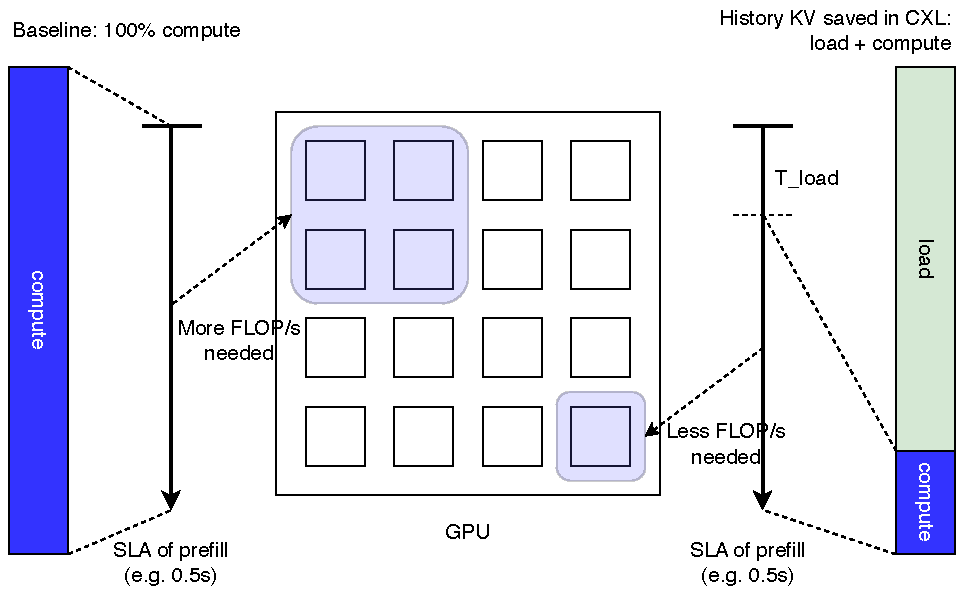
\includegraphics[width=0.48\textwidth]{fig/future/roi_explanation.pdf}
  %\end{top}
 \caption{Example of ROI modeling: replace computation with memory access}
    \label{fig:roi-modeling}
\end{wrapfigure}

By replacing computation with memory accesses, we reduce the overall computational load, thereby lowering the demand for FLOP/s while still meeting the same SLO. This results in significant cost savings for LLM inference (Figure~\ref{fig:roi-modeling}):

\begin{itemize}
\item \textbf{Assumption:} Assume a GPU has a computational power of 100 TFLOP/s, an average prefill request requires 25 TFLOP of computation, and the SLO for prefill is 0.5 seconds.
\item \textbf{Baseline:} To complete the prefill request within the SLO, each request demands 50 TFLOP/s (25 TFLOP/0.5s), meaning a single GPU can serve 2 prefill requests. 
\item \textbf{KVExpress:} By spending 0.1s loading KV cache data of the history context, we reduce the computational demand to 2.5 TFLOP (assuming the new prompt accounts for 10\%). To meet the same SLO, the remaining computation must be finished within 0.4s, requiring 6.25 TFLOP/s (2.5 TFLOP/0.4s). In this case, a single GPU can serve 16 prefill requests, yielding an \textbf{8x improvement over the baseline}.
\end{itemize}





This allows for a reduction of 87.5\% in the number of GPUs required for the same prefill SLO, resulting in substantial cost savings for LLM inference applications (more details in Appendix~\cite{roi_model}).


\begin{table}[ht]
    \caption{ROI Modeling}
    \label{tab:roi}
    \centering
    \small % Reduce font size
    \begin{tabularx}{\columnwidth}{lX}
        \hline
        $C_{0}$         & Avg. FLOPs needed by a prefill request in an initial request. Can be estimated as $C_{0}=2ML$, where $M$ is the model parameters and $L$ is the avg. sequence length. \\ \hline
        $C_{1}$         & FLOPs needed by new prompt in a follow-up request. Can be estimated as $C_{1}=rC_0$, where $r$ is the avg. ratio of the new prompt (e.g., 10\%). \\ \hline
        $T_{slo}$       & SLO of prefill (e.g., 0.5s). \\ \hline
        $T_{load}$      & Avg. time to load KV cache from memory (e.g., 0.1s). \\ \hline
        $P$             & Computation power (FLOP/s) of the GPU. \\ \hline
        $P_0$           & FLOP/s needed for the initial request. $P_{0} = C_{0}/T_{slo}$ \\ \hline
        $P_1$           & FLOP/s needed for the new prompt. $P_{1}=C_{1}/(T_{slo}-T_{load})$  \\ \hline
        $R_{gpu}$       & Request per second (RPS) a single GPU can support. $R_{gpu} = P/(P_{0}(1-h)+P_{1}h)$, where $h$ is the ratio of multi-round requests. \\ \hline
        $N_{cxl}$       & Number of GPUs needed using our CXL memory scheme. $N_{cxl} = \lceil R/R_{gpu} \rceil = \lceil \frac{R}{P/(P_{0}(1-h)+P_{1}h)} \rceil$ \\ \hline
        $N_{baseline}$  & Number of GPUs needed without any KV cache stored (i.e., all data discarded after prefill). $N_{baseline} = \lceil \frac{R}{P/P_0} \rceil$\\ \hline
    \end{tabularx}
\end{table}


\begin{comment}
\begin{table}
    \caption{ROI Modeling}
    \label{tab:roi}
    \centering
    \begin{tabular}{|l|p{4.5in}|}
$C_{0}$         & Avg. FLOPs needed by a prefill request in an initial request. Can be estimated as $C_{0}=2ML$, where $M$ is the model parameters and $L$ is the avg. sequence length. \\ \hline
$C_{1}$         & FLOPs needed by new prompt in an follow up request. Can be estimated as $C_{1}=rC_0$, where $r$ is the avg. ratio of the new prompt (e.g. 10\%). \\  \hline
$T_{slo}$       &  SLO of prefill (e.g. 0.5s).  \\  \hline
$T_{load}$      & Avg. time to load KV cache from memory (e.g. 0.1s). \\  \hline
$P$             & Computation power (FLOP/s) of the GPU. \\  \hline
$P_0$           & FLOP/s needed for the initial request. $P_{0} = C_{0}/T_{slo}$ \\  \hline
$P_1$           & FLOP/s needed for the new prompt. $P_{1}=C_{1}/(T_{slo}-T_{load})$  \\  \hline
$R_{gpu}$       & Request per second (RPS) a single GPU can support. $R_{gpu} = P/(P_{0}(1-h)+P_{1}h)$, where $h$ is the ratio of multi-round requests. \\  \hline
$N_{cxl}$       & Number of GPUs needed using our CXL memory scheme. $N_{cxl} = \lceil R/R_{gpu} \rceil = \lceil \frac{R}{P/(P_{0}(1-h)+P_{1}h)} \rceil$ \\  \hline
$N_{baseline}$  & Number of GPUs needed without any KV cache stored (i.e. all data discarded after prefill). $N_{baseline} = \lceil \frac{R}{P/P_0} \rceil$\\
    \end{tabular}
    
\end{table}
\end{comment}



\section{Conclusion}

\begin{comment}
\sam{
\begin{enumerate}
    \item recap problem and solution
    \item our prelim result
    \item future direction and promises (cache coherence in multi gpu?)
\end{enumerate}
}
\end{comment}

Storing KV caches in GPU memory for large language model (LLM) inference can quickly lead to memory saturation, limiting scalability and performance. To address this, we propose leveraging CXL memory, which offers expanded capacity with low-latency access, as a solution for offloading KV caches.

Our preliminary results show that CXL memory provides comparable performance to \ltp{traditional GPU memory in terms of latency, while also supporting larger workloads}. Specifically, using CXL memory for KV cache storage increased the maximum batch size by 30\%, from 44 to 57, while still meeting the same SLO. This demonstrates the potential for CXL memory to significantly reduce the computational burden on GPUs by offloading memory-intensive tasks.

Looking ahead, future work will explore the integration of CXL memory with multi-GPU systems, \ltp{focusing on maintaining cache coherence across GPUs}. This could further enhance the scalability and efficiency of LLM inference, unlocking new possibilities for large-scale AI workloads.

